% ============================================================
%  Experiment 2 --- DC Motor / PID Control (Position)
% ============================================================
\experimentheader{2}{Experiment 2}{DC Motor / PID Control --- Position}{Control Lab}

\begin{objectives}
  \begin{enumerate}
    \item To study open-loop position control of a DC motor.
    \item To study feedback (closed-loop) control using P, PI, PD, and PID controllers.
    \item To implement position control of a DC motor using a potentiometer and a resistance-to-voltage converter.
  \end{enumerate}
\end{objectives}

\begin{equipment}
  \begin{itemize}
    \item Controller kit
    \item Cathode ray oscilloscope
    \item BNC connectors with leads
    \item Multimeter
  \end{itemize}
\end{equipment}

\begin{procedure}

  \textbf{(a) Position control without feedback}
  \vspace*{1em}
  \begin{enumerate}
    \item Connect \textit{Output B} of the motor plant to Channel 2 of the oscilloscope.
    \item Connect \textit{Adjust A} of the motor plant to \textit{Input B} (position control) of the plant and to Channel 1 of the oscilloscope.
    \item Turn on the power switch.
    \item Slowly turn potentiometer-A clockwise ($0$ to $+50$) and anti-clockwise ($0$ to $-50$). Observe and describe the motor operation. Can you control the angular position of the motor?
    \item Turn off the motor by disconnecting \textit{Input B}.
  \end{enumerate}

  \begin{boxedfigure}
    \centering
    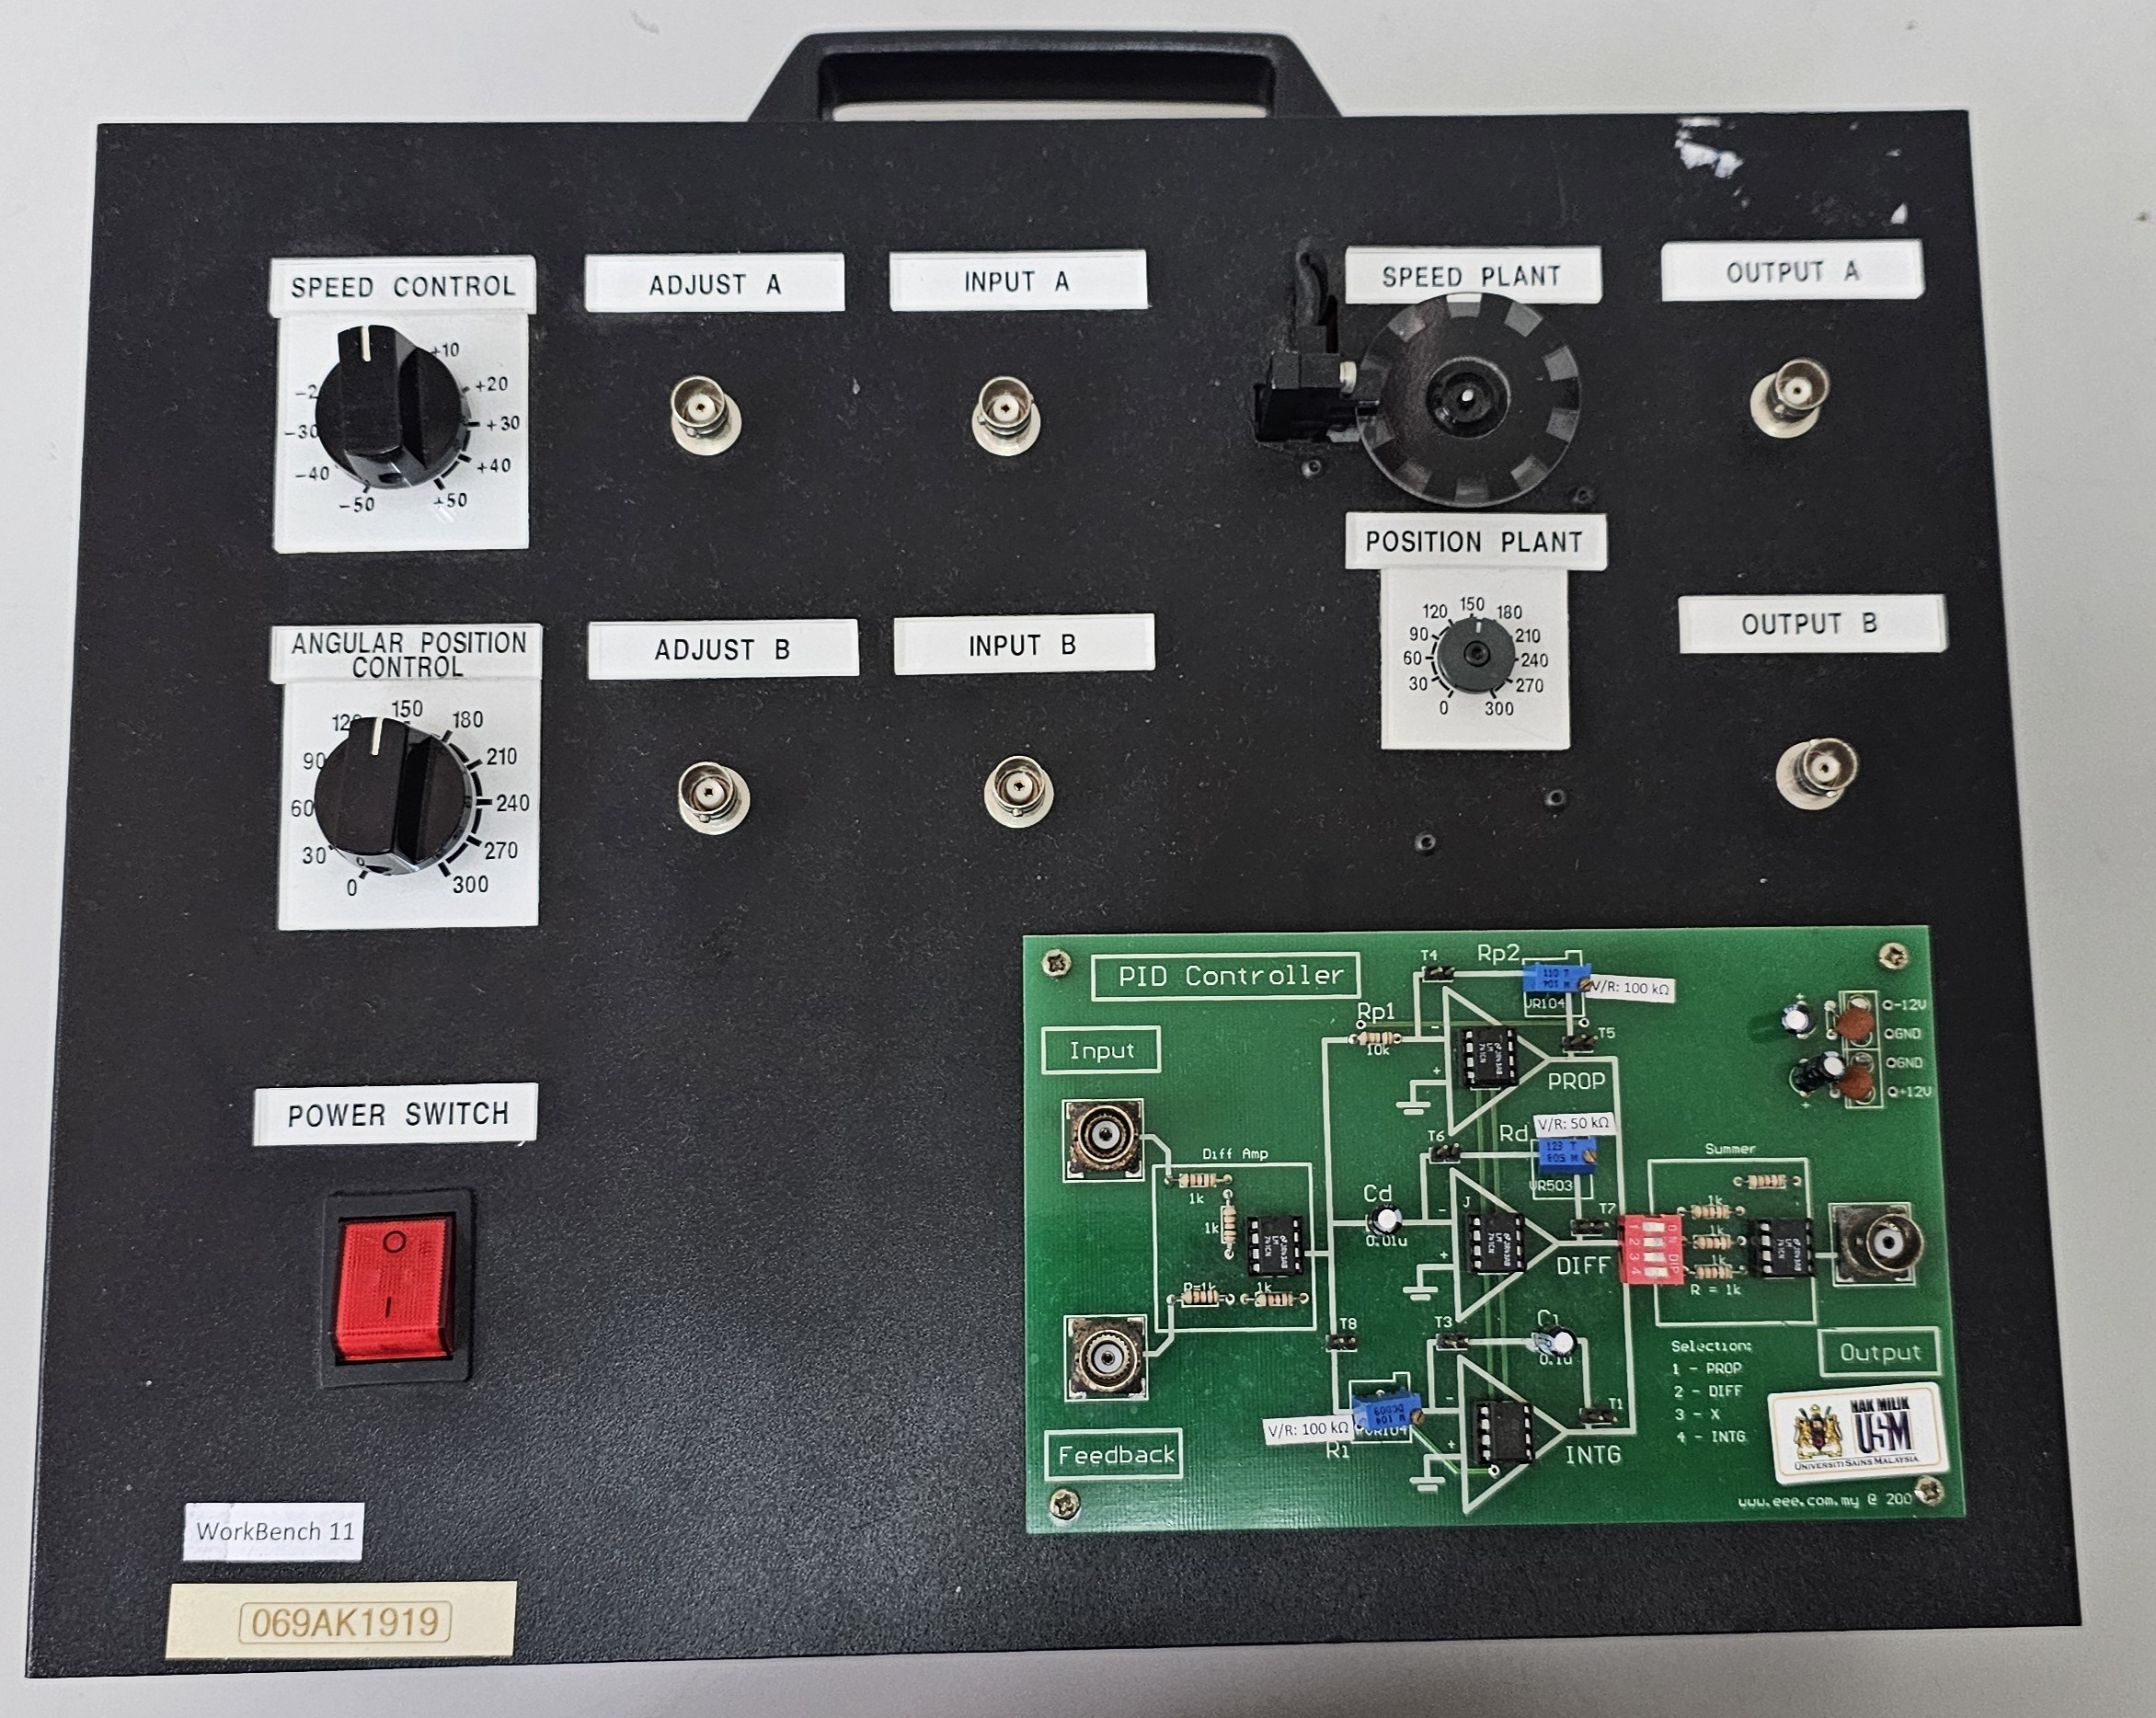
\includegraphics[width=0.85\linewidth]{figures/exp1-2-trainer.jpg}
    \captionof{figure}{DC Motor / PID Control trainer.}
    \label{fig:exp2-openloop}
  \end{boxedfigure}

  \textbf{(b) Closed-loop position control}
  \vspace*{1em}

  \textit{(i) Position control with proportional feedback control}\vspace{2pt}

  The motion of a motor can be converted into rotational position with the help of a suitable gearbox. The electrical signal, proportional to (angular) position, is obtained with the help of a circular potentiometer of good accuracy. \vspace*{1em}

  This signal is fed back to the summer to extract an error signal, which is fed to the controller to obtain optimum performance. Different controllers may be tried for this case, to study them: use the PID Controller daughterboard shown in Figure~\ref{fig:exp2-closedloop}, selecting the desired stage(s) via its DIP switch.

  \begin{boxedfigure}
    \centering
    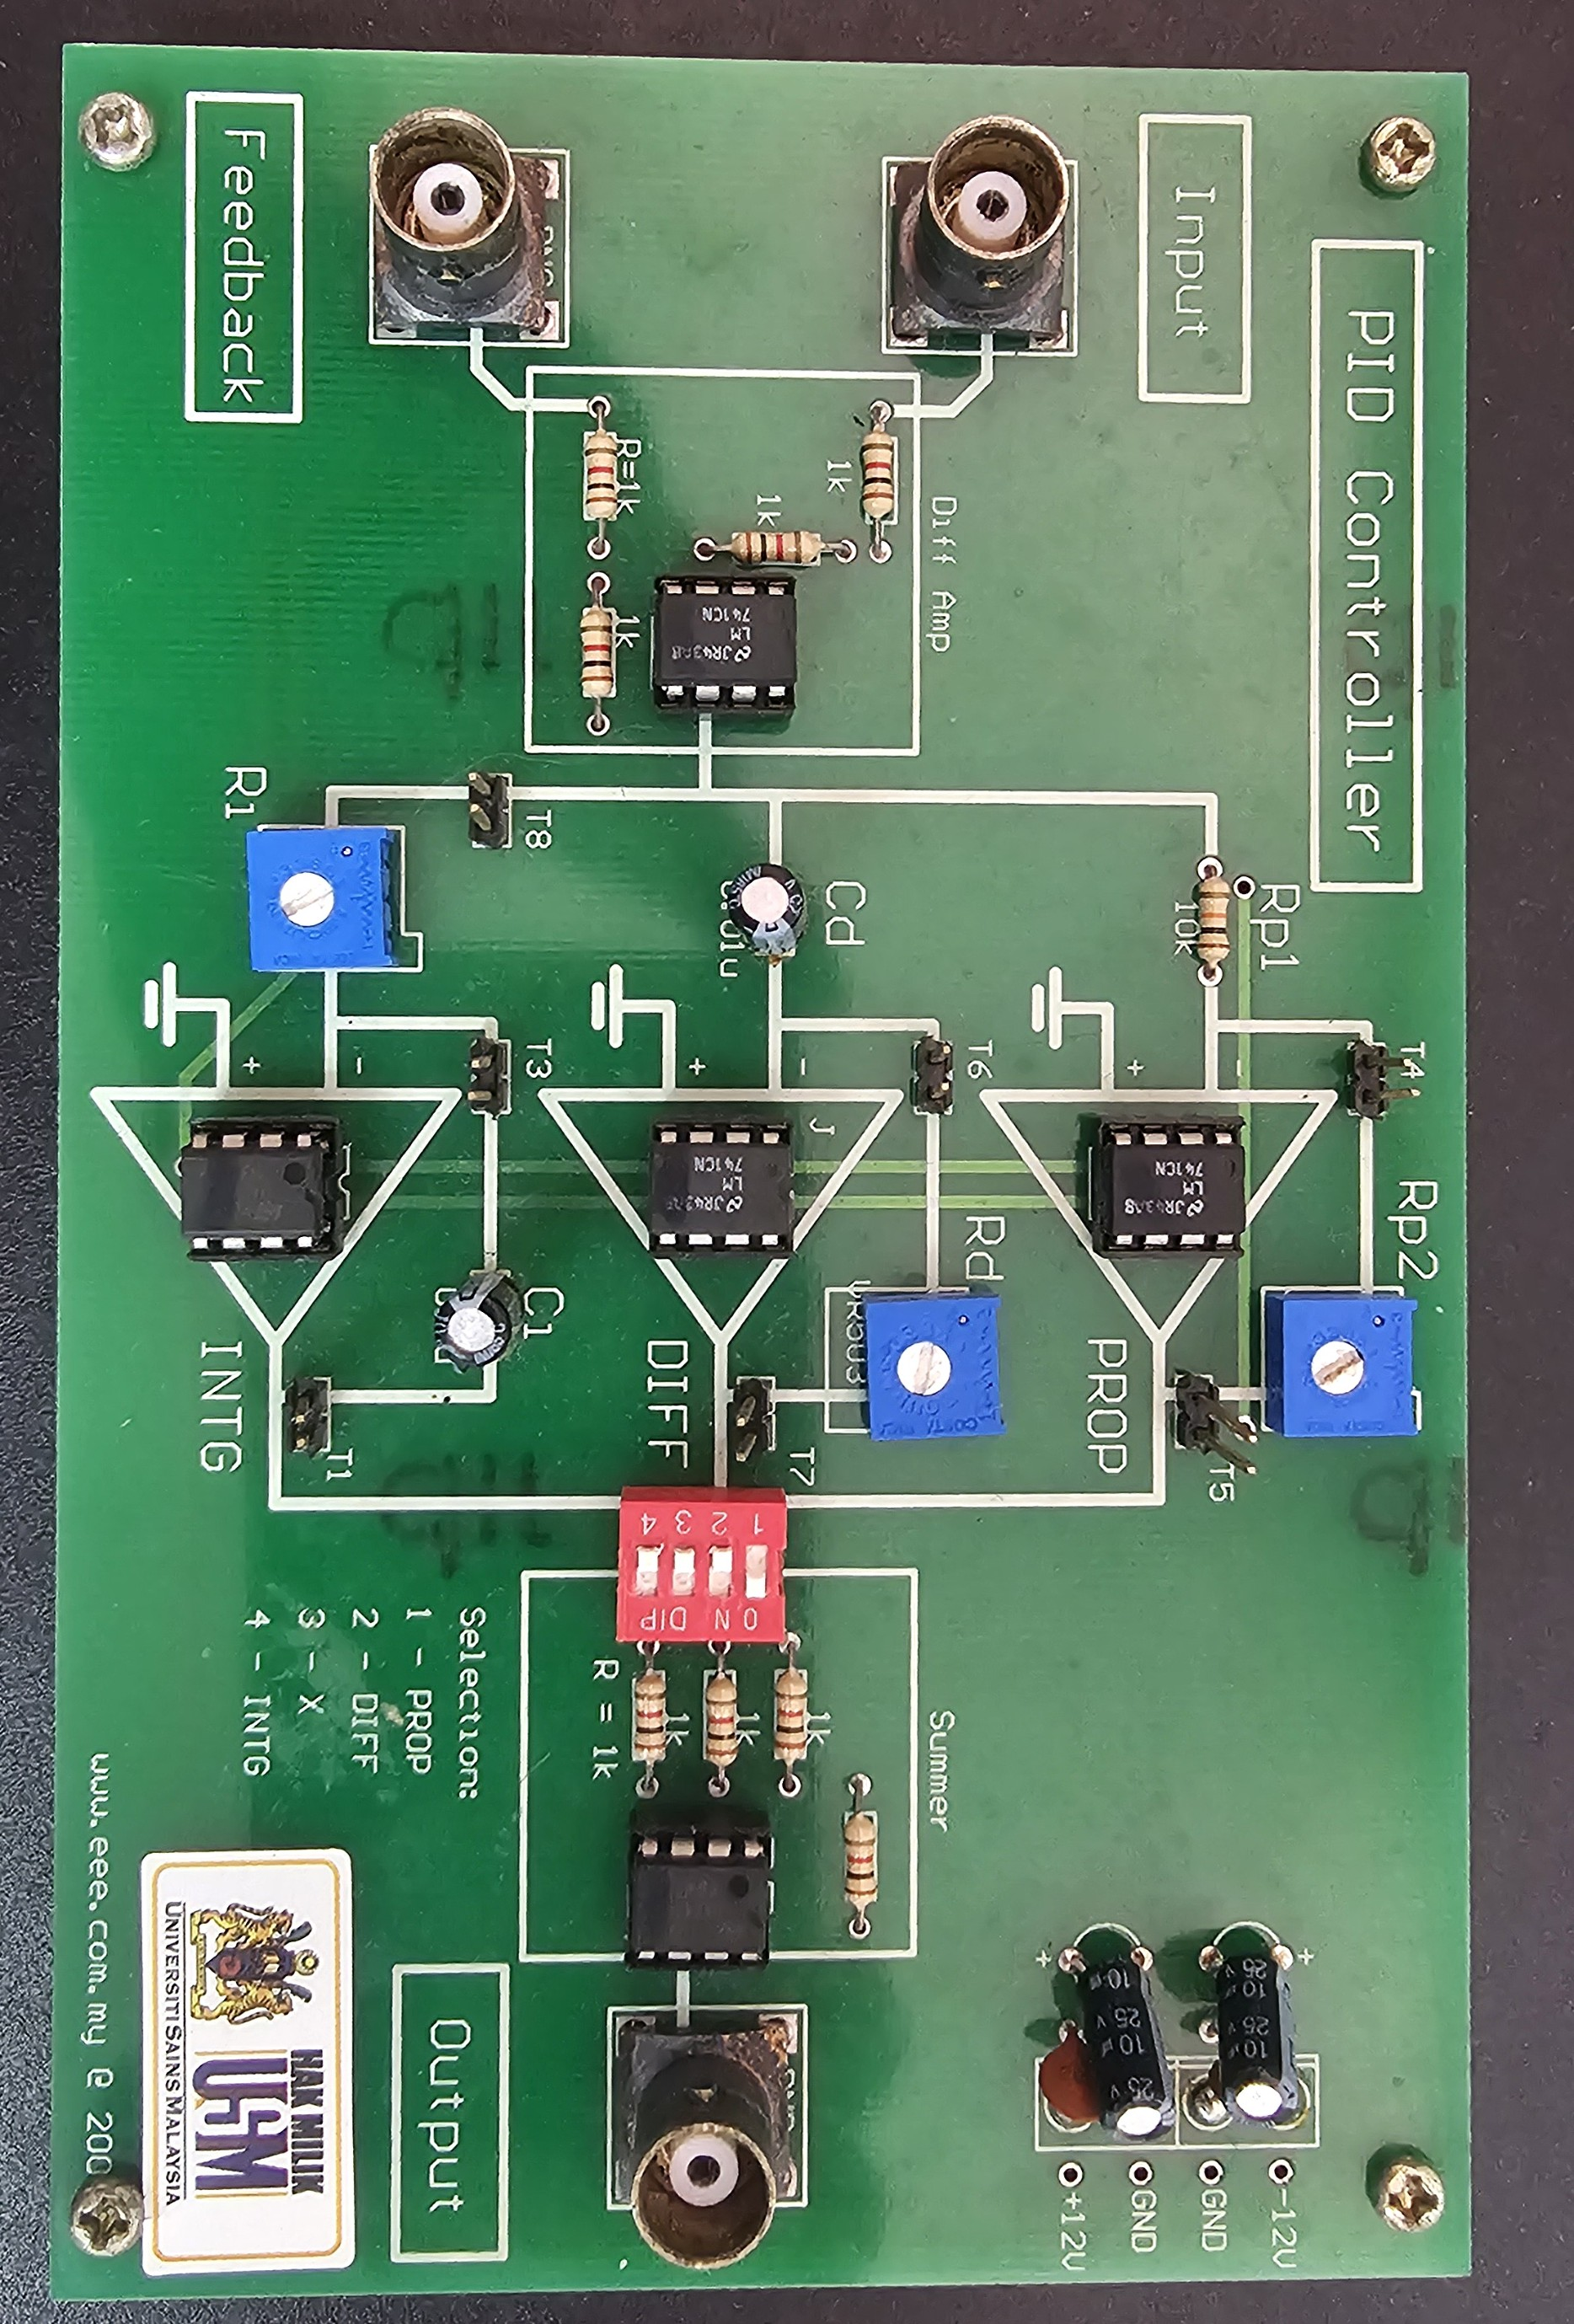
\includegraphics[width=0.6\linewidth, angle=90]{figures/exp1-2-controller.jpg}
    \captionof{figure}{PID Control module.}
    \label{fig:exp2-closedloop}
  \end{boxedfigure}

  \begin{enumerate}
    \item Select the P-controller by setting PROP on the controller (DIP switch 1) to ON; all other switches OFF.
    \item Connect \textit{Adjust B} of the plant to the \textit{input} of the PID controller.
    \item Connect \textit{Output B} of the plant to \textit{Feedback} of the controller.
    \item Connect the controller \textit{Output} to \textit{Input B} of the plant.
    \item Turn potentiometer-B of the motor plant to a middle position (e.g.\ $+180$).
    \item Adjust trimmer $R_{p2}$ (varying $K_p$) to obtain an optimum response (minimum steady-state error).
    \item Turn potentiometer-B to vary the position of the motor. Can the position be controlled in this case?
    \item Record the input and output voltages for various positions in Table~\ref{tab:exp2-table1}.
  \end{enumerate}

  \needspace{4cm}
  \begin{boxedtable}
    \captionof{table}{Position control response.}
    \label{tab:exp2-table1}
    {\renewcommand{\arraystretch}{1.5}%
      \centering
      \begin{tabular}{|c|c|c|c|c|}
        \hline
        Position & $V_{in}$ (Channel I) & $V_{out}$ (Channel II) & Error ($V_{out}-V_{in}$) & Remarks \\
        \hline
        $+270$   &                      &                        &                          &         \\
        \hline
        $+240$   &                      &                        &                          &         \\
        \hline
        $+210$   &                      &                        &                          &         \\
        \hline
        $+180$   &                      &                        &                          &         \\
        \hline
        $+150$   &                      &                        &                          &         \\
        \hline
        $+120$   &                      &                        &                          &         \\
        \hline
        $+90$    &                      &                        &                          &         \\
        \hline
        $+60$    &                      &                        &                          &         \\
        \hline
        $+30$    &                      &                        &                          &         \\
        \hline
      \end{tabular}
    }
  \end{boxedtable}
  \vspace*{1em}

  \textit{(ii) Position control with feedback and PI-controller}\vspace{2pt}

  \begin{enumerate}
    \item Select the PI-controller by setting PROP and INTG to ON.
    \item Connect \textit{Adjust B} of the plant to the \textit{input} of the PID controller.
    \item Connect \textit{Output B} of the plant to \textit{Feedback} of the controller.
    \item Connect the controller \textit{Output} to \textit{Input B} of the plant.
    \item Turn potentiometer-B of the motor plant to a middle position (e.g.\ $+180$).
    \item Slowly vary the respective trimmers $R_{p2}$ and $R_i$ to obtain an optimum output response.
    \item Turn potentiometer-B to vary the position of the motor. Record the input and output voltages for various positions.
  \end{enumerate}

  \textit{(iii) Position control with PD-controller}\vspace{2pt}

  \begin{enumerate}
    \item Select the PD-controller by setting PROP and DIFF to ON; all other switches OFF.
    \item Connect \textit{Adjust B} of the plant to the \textit{input} of the PID controller.
    \item Connect \textit{Output B} of the plant to \textit{Feedback} of the controller.
    \item Connect the controller \textit{Output} to \textit{Input B} of the plant.
    \item Turn potentiometer-B of the motor plant to a middle position (e.g.\ $+180$).
    \item Slowly vary the respective trimmers $R_{p2}$ and $R_d$ to obtain an optimum output response.
    \item Turn potentiometer-B to vary the position of the motor. Record the input and output voltages for various positions.
  \end{enumerate}
  \newpage

  \textit{(iv) Closed-loop control of position of motor using PID controller}\vspace{2pt}

  \begin{enumerate}
    \item Select the PID-controller by setting PROP, INTG, and DIFF to ON.
    \item Connect \textit{Adjust B} of the plant to the \textit{input} of the PID controller.
    \item Connect \textit{Output B} of the plant to \textit{Feedback} of the controller.
    \item Connect the controller \textit{Output} to \textit{Input B} of the plant.
    \item Turn potentiometer-B of the motor plant to a middle position (e.g.\ $+180$).
    \item Adjust the value of trimmers $R_{p2}$, $R_i$, and $R_d$ to obtain an optimum response (minimum steady-state error, quick operation, without overshoot or oscillations).
    \item Turn potentiometer-B to vary the position of the motor.
    \item Record the input and output voltages for various positions in Table~\ref{tab:exp2-table2}.
  \end{enumerate}

  \needspace{2cm}
  \begin{boxedtable}
    \captionof{table}{Closed-loop PID position response.}
    \label{tab:exp2-table2}
    {\renewcommand{\arraystretch}{1.5}%
      \centering
      \begin{tabular}{|c|c|c|c|c|}
        \hline
        Position & $V_{in}$ (Channel I) & $V_{out}$ (Channel II) & Error ($V_{out}-V_{in}$) & Remarks \\
        \hline
        $+270$   &                      &                        &                          &         \\
        \hline
        $+240$   &                      &                        &                          &         \\
        \hline
        $+210$   &                      &                        &                          &         \\
        \hline
        $+180$   &                      &                        &                          &         \\
        \hline
        $+150$   &                      &                        &                          &         \\
        \hline
        $+120$   &                      &                        &                          &         \\
        \hline
        $+90$    &                      &                        &                          &         \\
        \hline
        $+60$    &                      &                        &                          &         \\
        \hline
        $+30$    &                      &                        &                          &         \\
        \hline
      \end{tabular}
    }
  \end{boxedtable}

\end{procedure}

\begin{reportq}
  \begin{enumerate}
    \item Briefly explain the working of circuits used for the conversion of resistance to voltage.
    \item Describe in detail the applications of position control.
  \end{enumerate}
\end{reportq}
